\titreTD{\thenumTD}{Tableau p\'eriodique}
%##########################################################################
% Calcul de propri\'et\'es atomiques et mol\'eculaires
%##########################################################################
\exo{Utilisation du tableau p\'eriodique}
\begin{enumerate}[\bf 1)]
\item Quel est le symbole de l'atome ayant 45 protons?
\item Combien de protons poss\`ede le noyau de l'\'el\'ement argent?
\item Combien de protons et de neutrons poss\`ede le noyau d'h\'elium? Quelle est sa masse atomique?
\item L'\'el\'ement arsenic a un noyau ayant 33 protons. Combien l'\'el\'ement imm\'ediatement \`a sa droite dans le tableau
p\'eriodique poss\`ede-t-il de protons? Et celui imm\'ediatement \`a sa gauche? Et celui qui se trouve
4 colonnes avant?
\item Combien de proton poss\`ede le noyau du barium? Qu'en est-il de l'\'el\'ement imm\'ediatement \`a sa droite? Et celui d'apr\`es?
Combien y a-t-il d'\'el\'ements dans la p\'eriode qui d\'ebute par le C\'esium? Qu'en concluez-vous? Confirmez en refaisant la m\^eme travail pour
l'\'el\'ement dont le noyau poss\`ede 88 protons.
%%
\item L'oxyg\`ene, le soufre et le s\'el\'enium appartiennent au m\^eme groupe.
Quelle caract\'eristique ont-il en commun?
\item Quelle est la configuration \'electronique du carbone, du silicium, du germanium (Z=32),
de l'\'etain (Z=50) et du plomb (Z=82)?
Qu'en concluez-vous? Confirmez votre hypoth\`ese dans le groupe du Fluor.
\item Donnez la configuration \'electronique de l'atome d'oxyg\`ene neutre.
Combien a-t-il d'\'electrons de c\oe ur et de valence?
Le s\'el\'enium se trouve deux p\'eriodes sous l'atome d'oxyg\`ene.
Donnez sa configuration \'electronique de valence sans regarder le tableau.
\item Les questions suivantes doivent se faire sans regarder le tableau p\'eriodique.
\begin{enumerate}
\item Faites appara\^itre les blocs s, p et d sur le tableau p\'eriodique.
Attribuez \`a chacun d'eux une configuration \'electronique g\'en\'erique en appelant $n$ le num\'ero
de la p\'eriode.
\item De la m\^eme mani\`ere que dans la question pr\'ec\'edente, donnez la configuration \'electronique g\'en\'erique
des familles suivantes~: alcalins, alcalino-terreux, halog\`enes, gaz rares.
\item Le chlore est un halog\`ene de la troisi\`eme p\'eriode du tableau, quelle est sa configuration \'electronique de valence? M\^eme question pour le brome qui se trouve juste sous le chlore.
\item Le phosphore a la configuration \'electronique suivante $[Ne]3s^23p^3$. Quelle est la configuration
\'electronique de l'azote qui se trouve directement au-dessus du phosphore?
\end{enumerate}
%%
\item Quel est le rayon atomique du b\'eryllium (Z=4)? Et celui de l'\'el\'ement \`a sa gauche? Et \`a sa droite?
Comment ce rayon varie-t-il le long de la p\'eriode \`a laquelle appartient le b\'eryllium?
Faites le m\^eme travail pour la p\'eriode de l'\'el\'ement dont le noyau poss\`ede 22 protons.
La tendance observ\'ee est-elle g\'en\'erale?
\item On recherche les \'el\'ements ayant les caract\'eristiques suivantes~
\begin{enumerate}
\item forte \'electron\'egativit\'e/forme un sel avec un alcalin/pas le plus petit de son 
groupe/pas d'\'electrons $d$~;
\item perd facilement 2 \'electrons/pas d'\'electrons $d$/plus gros que le magn\'esium~;
\item configuration \'electronique de valence $3s^23p^1$/m\'etal~;
\item plus petit alcalin~;
\item alcalino-terreux de taille moyenne/des \'electrons $3d$ mais pas d'\'electron $4d$.
\end{enumerate}
\item Pointez cinq \'el\'ements sur le tableau p\'eriodique et donnez leurs configurations 
\'electroniques sans les lire.
\end{enumerate}
%
\exo{Configuration \'electronique}
\begin{enumerate}[\bf 1)]
\item \'Ecrire la configuration \'electronique atomique du zinc, dont le num\'ero 
atomique est Z=30.

\item Donner la configuration \'electronique et le nombre d'\'electrons non 
appari\'es, dans l'\'etat fondamental, des atomes suivants (en respectant le 
Principe de Pauli et en appliquant la r\`egle de Hund)~: N (Z=7), S (Z=16), 
Ca (Z=20), Fe (Z=26), Br (Z=35).

\item Dans les configurations \'electroniques suivantes d'un atome ou d'un ion, 
indiquer celles qui sont non-physiques (fausses), celles qui correspondent 
\`a un \'etat fondamental, et celles qui correspondent \`a un \'etat excit\'e.

\begin{center}
\begin{tabular}{lll}
$1s^1 2s^2 2p^1$ & $1s^2 2s^2 2p^3$ & $1s^2 2s^2 2p^6 3s^1 2d^{10}$         \\
$1s^2 2s^2 2p^2$ & $1s^3 2s^2 2p^4$ & $1s^2 2s^2 2p^6 3s^2 3p^6 4s^2 3d^1$  \\
\end{tabular}
\end{center}

\item Dans la classification p\'eriodique, les \'el\'ements allant du sodium 
(Z=11) au chlore (Z=17) ont une part de leur configuration \'electronique qui 
se retrouve pour chacun d'eux. Quel est l'\'el\'ement poss\'edant cette 
configuration~?  \'Ecrire, en se servant de cette observation, la structure 
\'electronique des deux \'el\'ements.

\item \'Etablir la configuration \'electronique de l'\'etat fondamental 
des atomes ou ions suivants~:

\begin{center}
\begin{tabular}{c|r}\hline
Z & charge \\\hline
11 & +1 \\\hline
17 & -1 \\\hline
18 & 0  \\\hline
19 & +1 \\\hline
\end{tabular}
\end{center}

Pour chacun d'eux donner le nombre d'\'electrons de valence.

\item D\'efinir halog\`ene, alcalin, m\'etal de transition, terres rares, gaz rare. 
Les situer dans le tableau p\'eriodique.

\end{enumerate}
%
\exo{Configuration \'electronique et classification p\'eriodique}
\begin{enumerate}[\bf 1)]
\item Soit l'\'el\'ement $_{31}^{69}$Ga. \'Ecrire sa configuration \'electronique atomique.
Dans quel bloc de la classification p\'eriodique se trouve cet \'el\'ement~?
Sur quelle p\'eriode~?
Dans quelle colonne~?
Est-ce un m\'etal~?
\item M\^emes questions pour les \'el\'ements $_{~6}^{12}$C, $_{15}^{31}$P, $_{20}^{40}$Ca, 
$_{22}^{48}$Ti, $_{32}^{71}$Ge et $_{38}^{88}$Sr.
\item Discutez l'\'evolution des propri\'et\'es m\'etalliques des sept \'el\'ements \'etudi\'es. 
Comparez les rayons atomiques des \'el\'ements appartenant \`a une m\^eme p\'eriode/\`a une m\^eme colonne.
\end{enumerate}
%--------------------------------------------
\exo{Orbitales et Cases Quantiques}
Le tableau p\'eriodique est rempli ligne apr\`es ligne (appel\'ees "p\'eriodes") en partant
de l'atome d'hydrog\`ene (Z=1). On peut d\'efinir des zones de remplissage correspondant \`a des
"orbitales". Pour cet exercice, on ne regarde qu'un raccourci du tableau.

\begin{center}
\begin{tabular}{rcllllllllllr}
1 & H  &    & & & &    &    &    &    &    & He & Couche K \\
2 & Li & Be & & & & B  & C  & N  & O  & F  & Ne & Couche L \\
3 & Na & Mg & & & & Al & Si & P  & S  & Cl & Ar & Couche M \\
\end{tabular}
\end{center}

\begin{enumerate}[\bf 1)]
\item Lien avec les couches K, L, M : La couche L correspond \`a la 2\textsuperscript{i\`eme} p\'eriode. Elle contient des
sous-couches et des orbitales. Nommez et dessinez les cases~quantiques associ\'ees aux orbitales de cette couche.
\item Les premi\`eres Orbitales Atomiques (OA) sont nomm\'ees $1s$ $2s$ $2p_x$ $2p_y$
2p$_z$. Les dessiner qualitativement ci-dessous dans la convention du cours (o\`u un signe positif est une
zone hachur\'ee et est conforme au rep\`ere). A titre d'exemple, l'orbitale $2p_x$ est dessin\'ee.
\end{enumerate}
%
\begin{center}
\begin{tabular}{ccccc}
\includegraphics[scale=0.6]{figure/repere_orbitale.eps} & \includegraphics[scale=0.6]{figure/repere_orbitale.eps} & \includegraphics[scale=0.6]{figure/orbitale.eps} & \includegraphics[scale=0.6]{figure/repere_orbitale.eps} & \includegraphics[scale=0.6]{figure/repere_orbitale.eps} \\
$1s$ & $2s$ & $2p_x$ & $2p_y$ & $2p_z$
\end{tabular}
\end{center}
%--------------------------------------------------------------------------
\exo{\'Etude des \'el\'ements des 1$^\textrm{er}$ et 2$^\textrm{e}$ groupes}
\begin{enumerate}[\bf 1)]
\item Nommez les \'el\'ements alcalins.
\item On donne la s\'erie des valeurs d'\'energies d'ionisation en kJ.mol$^{-1}$~: 375,6~; 402,9~; 418,7~; 495,7 et 520,1 pour ces \'el\'ements. Attribuez chaque valeur \`a un \'el\'ement, sachant qu'aucune valeur n'est donn\'ee pour le Francium. Expliquez la variation des \'energies d'ionisation dans la colonne.
\item \'Ecrire la structure \'electronique \underline{de valence} des \'el\'ements du 2$^\textrm{e}$ groupe.
\item Dites comment \'evoluent les grandeurs suivantes par rapport aux \'el\'ements alcalins~:
\begin{enumerate}%[~~~-]
\item degr\'e d'oxydation le plus souvent rencontr\'e,
\item dimension,
\item \'energie de premi\`ere ionisation.
\end{enumerate}
\end{enumerate}
%--------------------------------------------------------------------------
\exo{Propri\'et\'es des \'el\'ements et classification p\'eriodique}
\begin{enumerate}[\bf 1)]
\item \'Ecrire la structure \'electronique des ions suivants : I$^-$, Fe$^{2+}$, Cr$^{3+}$.
\item Classez les \'el\'ements suivants par ordre croissant de leur rayon atomique :
\begin{enumerate}%[~~~-]
\item Rb, Li, Na, K
\item Cl, Na, P, S, Mg, Si, Al
\end{enumerate}
\item Commentez la variation de l'\'electron\'egativit\'e dans le tableau p\'eriodique. Classez les \'el\'ements suivants par ordre d\'ecroissant d'\'electron\'egativit\'e : K, F, Na, Cl, I.
\end{enumerate}
%
\exo{D\'etermination d'un rayon m\'etallique}
Le sodium cristallise dans le r\'eseau cubique \`a faces centr\'ees, les atomes \'etant positionn\'es \`a chacun des sommets d'un cube et au centre de chaque face de ce m\^eme cube.
\begin{figure}[!h]
\begin{center}
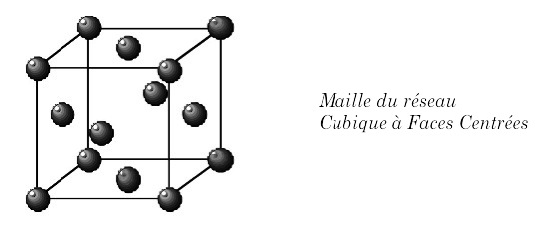
\includegraphics[scale=0.8]{figure/mailleCFC.eps}
\end{center}
\end{figure}
\begin{enumerate}[\bf 1)]
\item D\'eterminez le nombre d'atome de sodium par maille \'elementaire, en sachant que si un atome est partag\'e par $N$ mailles adjacentes, la maille \'el\'ementaire ne contient que $1/N$ atome.
\item Sachant que la masse volumique du sodium est de 968~kg/m$^3$, d\'eterminez le rayon m\'etallique $r_\textrm{Na}$.
On donne la constante d'Avogadro, $\mathcal{N}_a=6,022.10^{23}$mol$^{-1}$ et la masse atomique du sodium (22,990~g.mol$^{-1}$).
\end{enumerate}
%--------------------------------------------------------------------------
\exo{D\'etermination d'un rayon ionique}
NaCl cristallise dans le r\'eseau cubique faces centr\'ees repr\'esent\'e ci-dessous.\\
Examinez la structure et d\'eterminez le nombre d'ions Na$^+$ et Cl$^-$ dans la maille repr\'esent\'ee ci-dessous.
\begin{figure}[!h]
\begin{center}
\includegraphics[scale=0.6]{figure/cristalloNaCl.eps}
\end{center}
\end{figure}
\\Dans cet \'edifice, les anions et les cations sont en contact. 
La masse volumique d'un cristal de chlorure de sodium est de 2,163~g/cm$^3$. Le rayon ionique $r$(Cl$^-$) est de 1,81~\AA\ (voir Annexe).\\
Calculez, \`a l'aide de ces donn\'ees le rayon de l'ion Na$^+$. Comparez au rayon m\'etallique d\'etermin\'e dans l'exercice pr\'ec\'edent.\\
On donne la constante d'Avogadro, $\mathcal{N}_a=6,022.10^{23}$~mol$^{-1}$ et les masses atomiques du chlore (35,453~g.mol$^{-1}$), et du sodium (22,990~g.mol$^{-1}$).
%--------------------------------------------------------------------------
%\exo{\'Electron\'egativit\'e}
%On donne les affinit\'es \'electroniques $AE$, les \'energies d'ionisation $PI$, les \'energies de liaison homonucl\'eaire $E_\textsc{xx}$ et les \'energies de liaison avec l'hydrog\`ene $E_\textsc{hx}$ pour les \'el\'ements suivants :
%
%\begin{center}
%\begin{tabular}{|l|c|c|c|c|}\hline 
% & $AE$ (eV) & $PI$ (eV) & $E_\textsc{xx}$ (kJ/mol) & $E_\textsc{hx}$ (kJ/mol) \\\hline
%H & 0,75 & 13,60 & 435 & 435 \\\hline
%F & 3,45 & 17,42 & 158 & 570 \\\hline
%Cl & 3,61 & 13,01 & 243 & 431 \\\hline
%\end{tabular}
%\end{center}
%
%\begin{enumerate}%[\bf 1)]
%\item L'\'electron\'egativit\'e du fluor \'etant d\'efinie par $\chi_\textsc{f}=4.0$, calculez l'\'electron\'egativit\'e des autres \'el\'ements par la m\'ethode de Mulliken et par la m\'ethode de Pauling.\\
%Dans l'\'echelle de Mulliken, l'\'electron\'egativit\'e d'un \'el\'ement $X$ est donn\'ee par
%$$
%\chi_{_\textsc{x}}=k\left(\frac{PI_\textsc{x}+AE_\textsc{x}}{2}\right)\qquad \textrm{avec~}k=0.317\textrm{~eV}^{-1}
%$$
%
%\item Calculez l'\'energie de la liaison ClF.
%\end{enumerate}
%%--------------------------------------------------------------------------
%\exo{Moment dipolaire de mol\'ecules diatomiques}
%\begin{enumerate}%[\bf 1)]
%\item Sachant que pour LiH, le moment dipolaire exp\'erimental est de 5,9~D et que la longueur de liaison est de 1,60~\AA, calculez le pourcentage de caract\`ere ionique de la mol\'ecule.
%\item Calculez les pourcentages d'ionicit\'e des quatre halog\'enures d'hydrog\`ene connaissant la longueur de la liaison H-X et le moment dipolaire.
%\begin{center}
%\begin{tabular}{|l|c|c|c|c|}\hline 
%Halog\'enure d'hydrog\`ene & HF & HCl & HBr & HI \\\hline
%Moment Dipolaire $\mu$ en Debye (D)	& 1,82 & 1,07 & 0,79 & 0,38 \\\hline 
%Longueur de liaison en \AA & 0,92 & 1,27 & 1,41 & 1,61\\\hline
%\end{tabular}
%\end{center}
%\end{enumerate}
%\textbf{On rappelle~:} 1~D~=~3,33.10$^{-30}$~C.m et $e=\textrm{1,}602.10^{-19}$~C.
%%--------------------------------------------------------------------------
%\exo{Moment dipolaire d'une mol\'ecule coud\'ee}
%\begin{enumerate}%[\bf 1)]
%\item Donnez la structure de Lewis puis la g\'eom\'etrie de la mol\'ecule H$_2$S (S, atome central).
%\item Les \'electron\'egativit\'es du soufre et de l'hydrog\`ene sont respectivement~: 2,5 et 2,1 suivant l'\'echelle de Pauling. Donnez l'expression du moment dipolaire d'une des deux liaisons H–S sachant que le pourcentage de caract\`ere ionique de la liaison H–S est de 10\% et que sa longueur est de 135~pm.
%\item Calculez le moment dipolaire de H$_2$S, sachant que l'angle HSH vaut 92$\o$. Pr\'ecisez les charges port\'ees par chacun des atomes dans la mol\'ecule. 
%\end{enumerate}
%##########################################################################
% -- Exercice compl\'ementaire
%##########################################################################
\exo{D\'etermination d'un rayon ionique}
Calculez le rayon de l'ion Cs$^+$ en vous servant des donn\'ees suivantes : 
CsCl cristallise dans le r\'eseau cubique centr\'e, repr\'esent\'e ci-dessous.

\begin{figure}[!h]
\begin{center}
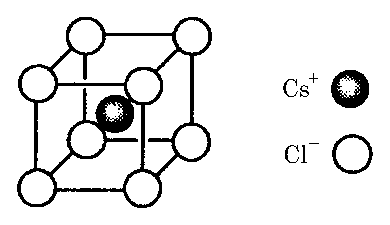
\includegraphics[scale=0.8]{figure/cristalloCsCl.eps}
\end{center}
\end{figure}

Dans cet \'edifice les anions et les cations sont en contact.\\
D\'eterminez le rayon ionique du cation Cs$^+$ sachant que la masse volumique du cristal de chlorure de c\'esium est de 3,990 g/cm$^3$ et le rayon ionique $r$(Cl$^-$) est de 1,81~\AA\ (voir Annexe).\\
On donne : $\mathcal{N}_a=6,022.10^{23}$mol$^{-1}$ ; $M$(Cl) = 35,453 g.mol$^{-1}$ ; $M$(Cs) = 132,905 g.mol$^{-1}$.
